\documentclass[prd,aps,10pt,nofootinbib,twocolumn,superscriptaddress,preprintnumbers,balancelastpage,longbibliography]{revtex4-1}

\usepackage{amsmath,amssymb}	
\usepackage{mathtools}
\usepackage{fontawesome}
\usepackage[dvipsnames]{xcolor}
\usepackage{hyperref}
\usepackage{xspace}
\usepackage{fancyhdr}
\usepackage{braket}
\usepackage{graphicx}
\usepackage{siunitx}
\usepackage{blindtext}
\usepackage{nicefrac}
\usepackage{lipsum}
\usepackage{bbold}

\usepackage{afterpage}
\newcolumntype{L}[1]{>{\raggedright\let\newline\\\arraybackslash\hspace{0pt}}m{#1}}
\newcolumntype{C}[1]{>{\centering\let\newline\\\arraybackslash\hspace{0pt}}m{#1}}
\newcolumntype{R}[1]{>{\raggedleft\let\newline\\\arraybackslash\hspace{0pt}}m{#1}}
\usepackage{longtable}
\setlength{\LTcapwidth}{\textwidth}

\newcommand{\nbicon}{{\color{linkcolor}\faFileCodeO}\xspace}
\newcommand{\nblink}[1]{\href{https://github.com/smsharma/dark-photons-perturbations/blob/apr-2020/notebooks/#1.ipynb}{\nbicon}}
\newcommand{\githubmaster}{\href{https://github.com/smsharma/dark-photons-perturbations/}{\faGithub}\xspace}

\newcommand{\dd}{\mathrm{d}}
\newcommand{\mAp}{m_{A^\prime}}
\newcommand{\vect}[1]{\boldsymbol{\mathbf{#1}}}

\definecolor{deepgreen}{rgb}{0.2,0.8,0.2}
\newcommand{\SM}[1]{{\bf \color{deepgreen}{[SM: #1]}}}

\colorlet{linkcolor}{BrickRed}



\hypersetup{colorlinks=true,
linkcolor=linkcolor,
citecolor=linkcolor,
urlcolor=linkcolor,
,linktocpage=true
,pdfproducer=medialab}

\DeclareSIUnit \h {\ensuremath{\mathit{h}}}
\DeclareSIUnit\electronvolt{e\kern-.05em V}
\DeclareSIUnit\parsec{pc}

\begin{document}

\title{A neural simulation-based inference approach for characterizing \\ the Galactic Center $\gamma$-ray excess}
 
\author{Siddharth Mishra-Sharma}
\email{sm8383@nyu.edu}
\thanks{ORCID: \href{https://orcid.org/0000-0001-9088-7845}{0000-0001-9088-7845}}
\affiliation{Center for Cosmology and Particle Physics, Department of Physics, New York University, New York, NY 10003, USA}

\author{Kyle Cranmer}
\email{kyle.cranmer@nyu.edu}
\thanks{ORCID: \href{https://orcid.org/0000-0002-5769-7094}{0000-0002-5769-7094}}
\affiliation{Center for Cosmology and Particle Physics, Department of Physics, New York University, New York, NY 10003, USA}
\affiliation{Center for Data Science, New York University, 60 Fifth Ave, New York, NY 10011, USA}

\date{\today}

\begin{abstract}
The nature of the \Fermi $\gamma$-ray Galactic Center Excess (GCE) has remained a persistent mystery for over a decade. Although the excess is broadly compatible with emission expected from dark matter annihilation, an explanation in terms of a population of unresolved point sources remains viable. The effort to uncover the origin of the GCE is hampered in particular by a poor understanding of diffuse emission of Galactic origin, which can lead to spurious features in the modeled data that make it difficult to robustly differentiate smooth emission, as expected due to a dark matter origin, from more ``clumpy'' emission expected from relatively bright, unresolved point sources. We use neural simulation-based inference methods, in particular conditional density estimation with normalizing flows, in order to extract more information from $\gamma$-ray maps of the Galactic Center with the aim of characterizing the contribution of unresolved point sources to the GCE. We do not find a preference in favor of a point source origin of the GCE within our framework.
\end{abstract}

\maketitle

\section{Introduction}
\label{sec:intro}

Dark matter (DM) represents one of the major unsolved problems in particle physics and cosmology today. The traditional Weakly-Interacting Dark Matter (WIMP) paradigm envisions production of dark matter in the early Universe through freeze-out of dark matter particles weakly coupled to the Standard Model (SM). In this scenario, one of the most promising avenues of detecting a dark matter signal would be through an observation of excess $\gamma$-ray photons from DM-rich regions of the sky produced through the cascade of SM particles resulting from DM self-annihilation. 

The \Fermi $\gamma$-ray Galactic Center Excess (GCE), first identified over a decade ago using data from the \Fermi Large Area Telescope (LAT)~\cite{Atwood:2009ez}, is an excess of photons in the Galactic Center with properties---such as energy spectrum and spatial morphology---broadly compatible with that expected due to annihilating DM~\cite{Goodenough:2009gk,Hooper:2010mq,Boyarsky:2010dr,Hooper:2011ti,Abazajian:2012pn,Hooper:2013rwa,Gordon:2013vta,Abazajian:2014fta,Daylan:2014rsa,Calore:2014xka,Abazajian:2014hsa,TheFermi-LAT:2015kwa,Linden:2016rcf,Macias:2016nev,Clark:2016mbb}. The nature of the GCE remains contentious however, with competing explanations in terms of a population of unresolved astrophysical point sources (PSs), in particular millisecond pulsars, remaining viable~\cite{Abazajian:2014fta,Abazajian:2010zy,Hooper:2013nhl,Calore:2014oga,Cholis:2014lta,Petrovic:2014xra,Yuan:2014yda,Brandt:2015ula}. Analyses of the spatial morphology of the excess have shown it to be more compatible with that tracing a stellar bulge distribution in the Galactic Center~\cite{Macias:2016nev,Macias:2019omb,Bartels:2017vsx}. Furthermore, analyses based on the statistics of photons in the Galactic Center have shown the data to prefer a point source origin of the excess~\cite{Lee:2015fea,Bartels:2015aea}. Recent studies have however pointed out the potential of unknown systematics---such as the poorly understood morphology of the diffuse foreground emission and unmodeled point sources---to bias these conclusions~\cite{Leane:2020nmi,Leane:2020pfc,Leane:2019xiy}.

 Due to the high dimensionality of $\gamma$-ray data, a hand-crafted reduction of the photon map into summaries such as the probability distribution of photon counts~\cite{Lee:2014mza,Lee:2015fea} or a wavelet decomposition~\cite{Balaji:2018rwz,McDermott:2015ydv} of the photon map has traditionally been necessary to enable computationally tractable analyses. On the other hand, recent developments in machine learning have given rise to analysis techniques that can extract more information from high-dimensional datasets and, consequently, more robustly hedge against unknown systematics in the data compared to traditional analyses based on specific data summaries. Machine learning methods have shown promise for analyzing $\gamma$-ray data~\cite{Caron:2021map} and in particular focusing on understanding the nature of the GCE~\cite{List:2020mzd,Caron:2017udl}. 
 
 In this paper, we leverage recent developments in the field of simulation-based inference (SBI; see, \emph{e.g.}, Ref.~\cite{cranmer2020frontier} for a review)~\cite{Alsing:2019xrx,Brehmer:2018eca,Brehmer:2018hga,Brehmer:2018kdj,Brehmer:2020cvb,Cranmer:2015bka,cranmerFrontierSimulationbasedInference2020,durkanContrastiveLearningLikelihoodfree2020,greenbergAutomaticPosteriorTransformation2019,Hermans:2019ioj,lueckmannBenchmarkingSimulationBasedInference2021,lueckmannLikelihoodfreeInferenceEmulator2019,pacchiardiGeneralizedBayesianLikelihoodFree2021,papamakariosFastEpsilonFree2018,papamakariosSequentialNeuralLikelihood2019,wiqvistSequentialNeuralPosterior2021,zhaoValidatingConditionalDensity2021} in order to weigh in on the nature of the GCE. In particular, we employ conditional density estimation techniques based on normalizing flows~\cite{papamakarios2019normalizing,rezende2015variational} in order to characterize the contributions of various modeled components, including ``clumpy'' PS-like and ``smooth'' DM-like emission following the GCE, to the $\gamma$-ray photon sky at $\sim$GeV energies in the Galactic Center. We employ graph neural networks in order to automatically extract summary statistics from $\gamma$-ray maps optimized for the downstream task of estimating the parameter posteriors of various components characterizing the GCE.

This paper is organized as follows. In Sec.~\ref{sec:analysis} we describe the various components of our analysis method based on simulation-based inference. In Sec.~\ref{sec:simulations} we describe our simulation pipeline and verify our analysis on simulated data. Section~\ref{sec:data} presents results on \Fermi $\gamma$-ray data. In Sec.~\ref{sec:mismodeling} we explore the susceptibility of the analysis to mismodeling of the background and signal templates, and present systematic variations on our analysis in Sec.~\ref{sec:systematics}. We conclude in Sec.~\ref{sec:conclusion}.

\section{Methodology}
\label{sec:analysis}

We begin by describing our analysis methodology, going over in turn the general principles behind simulation-based inference, posterior estimation using normalizing flows, and learning representative summary statistics from high-dimensional $\gamma$-ray maps with neural networks. We then describe the various components that go into our forward model and the datasets used, concluding with an outline of our optimization procedure.

\subsection{Simulation-based inference}

Of central interest in parameter estimation is often the probability distribution of a set of parameters of interest $\theta$ given some data $x$---the posterior distribution $p(\theta\mid x)$. Bayes' theorem can be used to obtain the posterior as $p(\theta\mid x) = p(\theta)\, p(x\mid\theta) / \mathcal Z$, where $p(x\mid\theta)$ is the likelihood and $\mathcal Z$ is the Bayesian evidence. In practice, parameters other than $\theta$---latent variables $z$---are often involved in the data-generation process, and computing the likelihood involves marginalizing over the latent space, $p(x\mid\theta) = \int \dd z\,p(x\mid\theta, z)$. In typical problems of interest, the high dimensionality of the latent space often means that this integral is intractable, necessitating simplifications in statistical treatment as well as theoretical modeling. 

% $\theta \sim p(\theta)$, $x\sim p(x\mid\theta, z)$, $z\sim p(z\mid\theta)$.

Simulation-based inference (SBI) refers to a class of methods for performing inference when the data-generating process does not have a tractable likelihood. In this setting, a model is defined through a simulator as a probabilistic program, often knows as a forward model. Samples $x$ from the simulator then implicitly define a likelihood, $x\sim p(x\mid\theta)$. In the simplest realizations of SBI, samples $x'$ generated from a given prior proposal distribution $p(\theta$) can be compared to a given dataset of interest $x$, with the approximate posterior defined by samples that most closely approximate $x$ according to some distance metric. Such methods---usually grouped under the umbrella of Approximate Bayesian Computation (ABC)~\cite{10.1214/aos/1176346785}---are not uncommon in astrophysics and cosmology. Nevertheless, they suffer from several downsides. The curse of dimensionality usually necessitates reduction of data to representative lower-dimensional summary statistics $s(x)$, resulting in loss of information. A notion and measure of distance between summaries from the implicit model and those derived from the dataset of interest is necessary, leading to inexact inference. Additionally, the ABC analysis must be performed anew for each new target dataset.

Recent methods have leveraged advancements in machine learning, in particular the ability of neural networks to extract useful features from high-dimensional data and flexibly approximate functions and distributions, in order to address these issues, enabling new ways of performing inference on complex models defined through simulations (see Ref.~\cite{cranmer2020frontier} for a review of recent developments).

\subsection{Conditional density estimation with normalizing flows}

In this paper, we approximate the joint posterior $p(\theta\mid x)$ through a parameterized distribution $\hat p_\phi(\theta\mid s)$ conditioned on \emph{learned} summaries $s=s(x)$ from the simulated samples $x$. This class of simulation-based inference techniques, known as conditional neural density estimation~\cite{papamakariosFastEpsilonFree2018}, directly models the posterior distribution given a set of samples drawn from simulator drawns according to some prior proposal distribution $p(\theta)$.

We employ normalizing flows~\cite{papamakarios2019normalizing,rezende2015variational}, which provide an efficient way of constructing flexible probability distributions. Normalizing flows model the conditional distribution $\hat p_\phi(\theta\mid s)$ as a series of invertible transformations, denoted $f$ and having a tractable inverse and Jacobian, from a base distribution $\pi_z({z})$, chosen here to be a standard Gaussian $z\sim \mathcal N(0, \mathbb{1})$, to the target distribution:
\begin{equation}
    \hat{p}({\theta} \mid {x})=\pi_{z}\left(f^{-1}({\theta})\right)\left|\operatorname{det}\left(\frac{\partial f^{-1}}{\partial {\theta}}\right)\right|
\end{equation}
Specifically, we use Masked Autoregressive Flows (MAFs)~\cite{10.5555/3294771.3294994} for posterior estimation. The MAF is built upon blocks of affine transformations where the scaling and shifting factors for each dimension are computed with a Masked Autoencoder for Distribution Estimation (MADE)~\cite{germain2015made}. For a single block, the transformation is expressed as 
\begin{equation}
    \label{eq:maf_z}
    z_{i}=\left(\theta_{i}-\mu_{i}\right) \cdot \exp \left(-\alpha_{i}\right)
\end{equation}
where $\mu_{i}=f_{\mu_{i}}\left({\theta}_{1: i-1} ; {x}\right)$ and $\alpha_i = f_{\alpha_{i}}\left({\theta}_{1: i-1} ; {x}\right)$ are scaling and shift factors modeled by a MADE according to the autoregressive condition. This allows for an analytically tractable determinant,
\begin{equation}
    \label{eq:det}
    \left|\operatorname{det}\left(\frac{\partial f^{-1}}{\partial {\theta}}\right)\right|=\exp \left(-\sum_{i} \alpha_{i}\right)
\end{equation}
and a forward pass through the flow according to Eq.~\eqref{eq:maf_z}.
Multiple transformations can be composed together as $f=f_{1} \circ f_{2} \circ \ldots \circ f_{K}$ in order to model more expressive posteriors,
\begin{equation}
    \hat{p}({\theta} \mid {x})=\pi_{z}\left(f^{-1}({\theta})\right) \prod_{i=1}^{K}\left|\operatorname{det}\left(\frac{\partial f_{i}^{-1}}{\partial {z}_{i-1}}\right)\right|.
\end{equation}
The log-probability of the posterior can then be computed using Eq.~\eqref{eq:det}:
\begin{equation}
    \log \hat{p}({\theta} \mid {x}) = \log \left[\pi_{z}\left(f^{-1}(\boldsymbol{\theta})\right)\right]-\sum_{i=1}^{K} \sum_{j=1}^{N} \alpha_{j}^{i},
\end{equation}
which acts as the optimization objective. Here, we use 8 MAF transformations, each made up of a 2-layer MADE with 128 hidden units. Each MAF transformation is conditioned on summaries $s(x)$  extracted from the $\gamma$-ray maps (described below) by including these as inputs into each transformation block.

\subsection{Learning summary statistics with neural networks}

The curse of dimensionality makes it computationally prohibitive to condition the density estimation task on the the raw dataset $x$ \emph{i.e.}, the $\gamma$-ray pixel counts map in the region of interest (ROI). Representative summaries $s = s_\varphi(x)$ of the data must therefore be extracted in order to enable a tractable analysis. Although many choices for data summaries are possible---\emph{e.g.}, a Principal Component Analysis (PCA) decomposition of the photon counts map, an angular power spectrum decomposition of the photon counts map, or simply a histogram of the photon counts---in this paper, we use a neural net to automatically learn low-dimensional summaries that are efficiently suited for the specific downstream task at hand.

The \emph{DeepSphere}~\cite{defferrard2020deepsphere,Perraudin:2018rbt} architecture, with a configuration similar to that introduced and first employed in Ref.~\cite{List:2020mzd} for the purpose of analyzing \Fermi data in the Galactic Center region, is used and summarized briefly here. \emph{DeepSphere} is a graph-based convolutional neural network (CNN) architecture tailored to data sampled on a sphere, and in particular is able to leverage the hierarchical structure of data in the \texttt{HEALPix} representation. This makes it well-suited for our purposes.

The \texttt{HEALPix} sphere is represented as a weighted undirected graph $\mathcal G = (\mathcal V, \mathcal E, \boldsymbol A)$.  where $\mathcal V$ is the set of $N_\mathrm{pix} = |\mathcal V|$ vertices, $\mathcal E$ is the set of edges, and $\boldsymbol A$ is the weighted adjacency matrix. Each pixel $i$ is represented by a vertex $v_i \in \mathcal V$. Each vertex $v_i$ is then connected to the 8 (or 7) vertices $v_j$ which represent the neighboring pixels $j$ of pixel $i$, forming edges $(v_i
, v_j) \in \mathcal E$. Given those edges, we define the weights of the adjacency matrix $\boldsymbol A$ over neighboring pixels following the weighing scheme given in Ref.~\cite{defferrard2020deepsphere}.

The combinatorial graph Laplacian is defined as $\boldsymbol L = \boldsymbol D - \boldsymbol A$, where $\boldsymbol D$ is the diagonal degree matrix, and can be used to define a Fourier basis on a graph. By construction symmetric positive semi-definite, the graph Laplacian can be decomposed as $\boldsymbol L = \boldsymbol U \boldsymbol \Lambda \boldsymbol U^T$, where $\boldsymbol U$ is an orthonormal eigenvectors matrix and $\boldsymbol \Lambda$ is a diagonal eigenvalue matrix. The Laplacian eigenvectors then define the graph Fourier basis, with the graph Fourier transform $\hat{\boldsymbol x}$ of a signal $\boldsymbol x$ on a graph being its projection $\hat{\boldsymbol x} = \boldsymbol U^T \mathbf x$.

Given a convolutional kernel $h$, graph convolutions can be performed in the Fourier basis as $h(\boldsymbol{L}) \boldsymbol{x}=\boldsymbol{U} h(\boldsymbol{\Lambda}) \boldsymbol{U}^{\top} \boldsymbol{x}$.

The convolutional kernel $h$ is defined as Chebychev polynomials $h_{\theta}({\boldsymbol{L}}) = \sum_{k=0}^{K} \theta_{k} T_{k}({\boldsymbol{L}})$ of degree $K$ parameterized by $K + 1$ coefficients $\theta$. The graph filering operation can then be expressed as
\begin{equation}
    h_{\theta}(\boldsymbol{L}) \boldsymbol{x}=\boldsymbol{U}\left(\sum_{k=0}^{K} \theta_{k} T_k(\boldsymbol{\Lambda})\right) \boldsymbol{U}^{\top} \boldsymbol{x}=\sum_{k=0}^{K} \theta_{k} T_k(\boldsymbol{L}) \boldsymbol{x},
\end{equation}
where $T_k$ is the order-$k$ Chebyshev polynomial and $\theta_k$ are the filter coefficients to be optimized. $K=9$ is the maximum polynomial order used in our fiducial configuration.

Following Ref.~\cite{Perraudin:2018rbt}, our feature extraction architecture is built out of layers which progressively coarsen the pixel representation of the $\gamma$-ray maps while increasing the number of filter channels at each step. Starting with \HEALPix resolution \texttt{nside}=128, each graph convolution operation is followed by a BatchNorm, a ReLU nonlinearity, and a max pooling operation which downsamples the representation into a coarser resolution, starting with \texttt{nside}=64 until resolution \texttt{nside}=1 after the final convolutional layer. The number of filter channels is doubled at each convolution until a maximum of 256. The final convolution is flattened and passed through a fully-connected layer with 2048 hidden units before output a desired number of summaries, which is 128 in our fiducial configuration.

\subsection{Datasets and the forward model}
\label{sec:datasets}

We use the datasets and templates from Ref.~\cite{rodd_nicholas_safdi_siddharth_2016} (packaged with Ref.~\cite{Mishra-Sharma:2016gis}) to create the simulated maps for forward modeling. The data and templates used correspond to 413 weeks of \emph{Fermi}-LAT Pass 8 data collected between August 4, 2008 and July 7, 2016. The top quarter of photons in the energy range 2--20~GeV by quality of PSF reconstruction (corresponding to PSF3 event type) in the event class \texttt{ULTRACLEANVETO} are used. The recommended quality cuts are applied, corresponding to zenith angle less than 90$^\circ$, \texttt{LAT\_CONFIG} = 1, and \texttt{DATA\_QUAL} $> 0.1$.\footnote{\url{https://fermi.gsfc.nasa.gov/ssc/data/analysis/documentation/Cicerone/Cicerone_Data_Exploration/Data_preparation.html}} The maps are spatially binned using \texttt{HEALPix}~\cite{Gorski:2004by} with \texttt{nside}=128.

The simulated data maps are a combination of smooth (\emph{i.e.}, Poissonian) and PS contributions. Each PS population is completely specified by its spatial distribution, described by a spatial template, and the distribution of photon counts, specified by a source-count distribution. PS populations spatially correlated with \emph{(i)}~the GCE, modeled using a squared-NFW profile with inner slope $\gamma=1.2$ motivated by previous GCE analysis,
\begin{equation}
    \rho(r) \propto \frac{1}{\left(r / r_{s}\right)^{\gamma}\left(1+r / r_{s}\right)^{3-\gamma}}
\end{equation}
where $r_{s}=20\,\mathrm{kpc}$ is the Milky Way scale radius, and \emph{(ii)}~the Galactic disk, modeled as a doubly-exponential profile,
\begin{equation}
    n(R, z) \propto \exp (-R / 5\,\mathrm{kpc}) \exp (-|z| / 1\,\mathrm{kpc})
\end{equation}
where R and z are the radial and vertical Galactic cylindrical coordinates. Variations on these choices are explored in the Appendix. Photon counts from a generated PS population are put down on a map according to the \emph{Fermi} PSF at 2 GeV, modeled as a King function, using the algorithm implemented in the code package \texttt{NPTFit-Sim}~\cite{NPTFit-Sim}. The source-count distribution $\dd N /\dd S$ of each PS population is modeled as a doubly-broken power law,
\begin{equation}
    \frac{d N_{p}}{d S}=A\left\{\begin{array}{lc}
        \left(\frac{S}{S_{b, 1}}\right)^{-n_{1}}, & S \geq S_{b, 1} \\
        \left(\frac{S}{S_{b, 1}}\right)^{-n_{2}}, & S_{b, 1}>S \geq S_{b, 2} \\
        \left(\frac{S_{b, 2}}{S_{b, 1}}\right)^{-n_{2}}\left(\frac{S}{S_{b, 2}}\right)^{-n_{3}}, & S_{b, 2}>S
        \end{array}\right.
\end{equation}
specified by the breaks $\{S_{b, 1}, S_{b, 2}\}$, slopes $\{n_1, n_2, n_3\}$, and an overall normalization $A$. We note that these parameters specify the \emph{spatially-averaged} properties of the PS population---variation due to non-uniform exposure of the LAT instrument is accounted for in putting down simulated counts.

In addition to the PS-like emission, we account for Poissonian astrophysical emission in the simulated maps.  These contributions include: \emph{(i)}~the Galactic diffuse foreground emission, described in the baseline case by \texttt{Model~O} from Ref.~\cite{Buschmann:2020adf}, \emph{(i)}~DM-like emission following a generalized squared-NFW profile with $\gamma=1.2$, \emph{(iii)}~isotropic emission, \emph{(iv)}~resolved PSs from the 3FGL catalog, and \emph{(v)}~emission from the \Fermi bubbles~\cite{Su:2010qj}. The latter three templates are obtained from Ref.~\cite{rodd_nicholas_safdi_siddharth_2016}. The final maps are obtained by combining a Poisson-fluctuated realization of the combined astrophysical templates with the PS maps. The inner regions of the Galactic plane are masked at $|b| < 2^\circ$, and a radial cut $r < 25^\circ$ defines the region of interest for the fiducial analysis. We mask resolved PSs from the 3FGL catalog at a containment radius of $0.8^\circ$.   

The forward model is thus specified by 18 parameters---6 parameters for the overall normalizations of the Poissonian templates, and $6\times2$ parameters modeling the source-count distribution associated with GCE-correlated and disk-correlated PS populations. Simulated samples are produced using parameters drawn from priors motivated by a Poissonian fit to the real \Fermi data in order to improve sample efficiency. Since PS-like and Poissonian components of the model are exactly degenerate in the limit of dim sources, we place priors on the expected counts contribution per pixel for the GCE-correlated PS-like and Poissonian emission in order to mitigate biases caused by an induced prior preferring one model over the other and preventing the expression of the degeneracy.

\subsection{Optimization and training}

$10^{6}$ training samples are generated. Models are trained with batch size 128 using the \texttt{AdamW} optimizer with initial learning rate $10^{-3}$ and weight decay $10^{-5}$. Cosine annealing is used to decay the learning rate, training for up to 100 epochs with early stopping if the validation loss has not improved after 10 epochs. All input features (\emph{i.e.}, individual pixels as well as auxiliary variables) are normalized to zero mean and unit variance.

%
\begin{figure*}
    \centering
    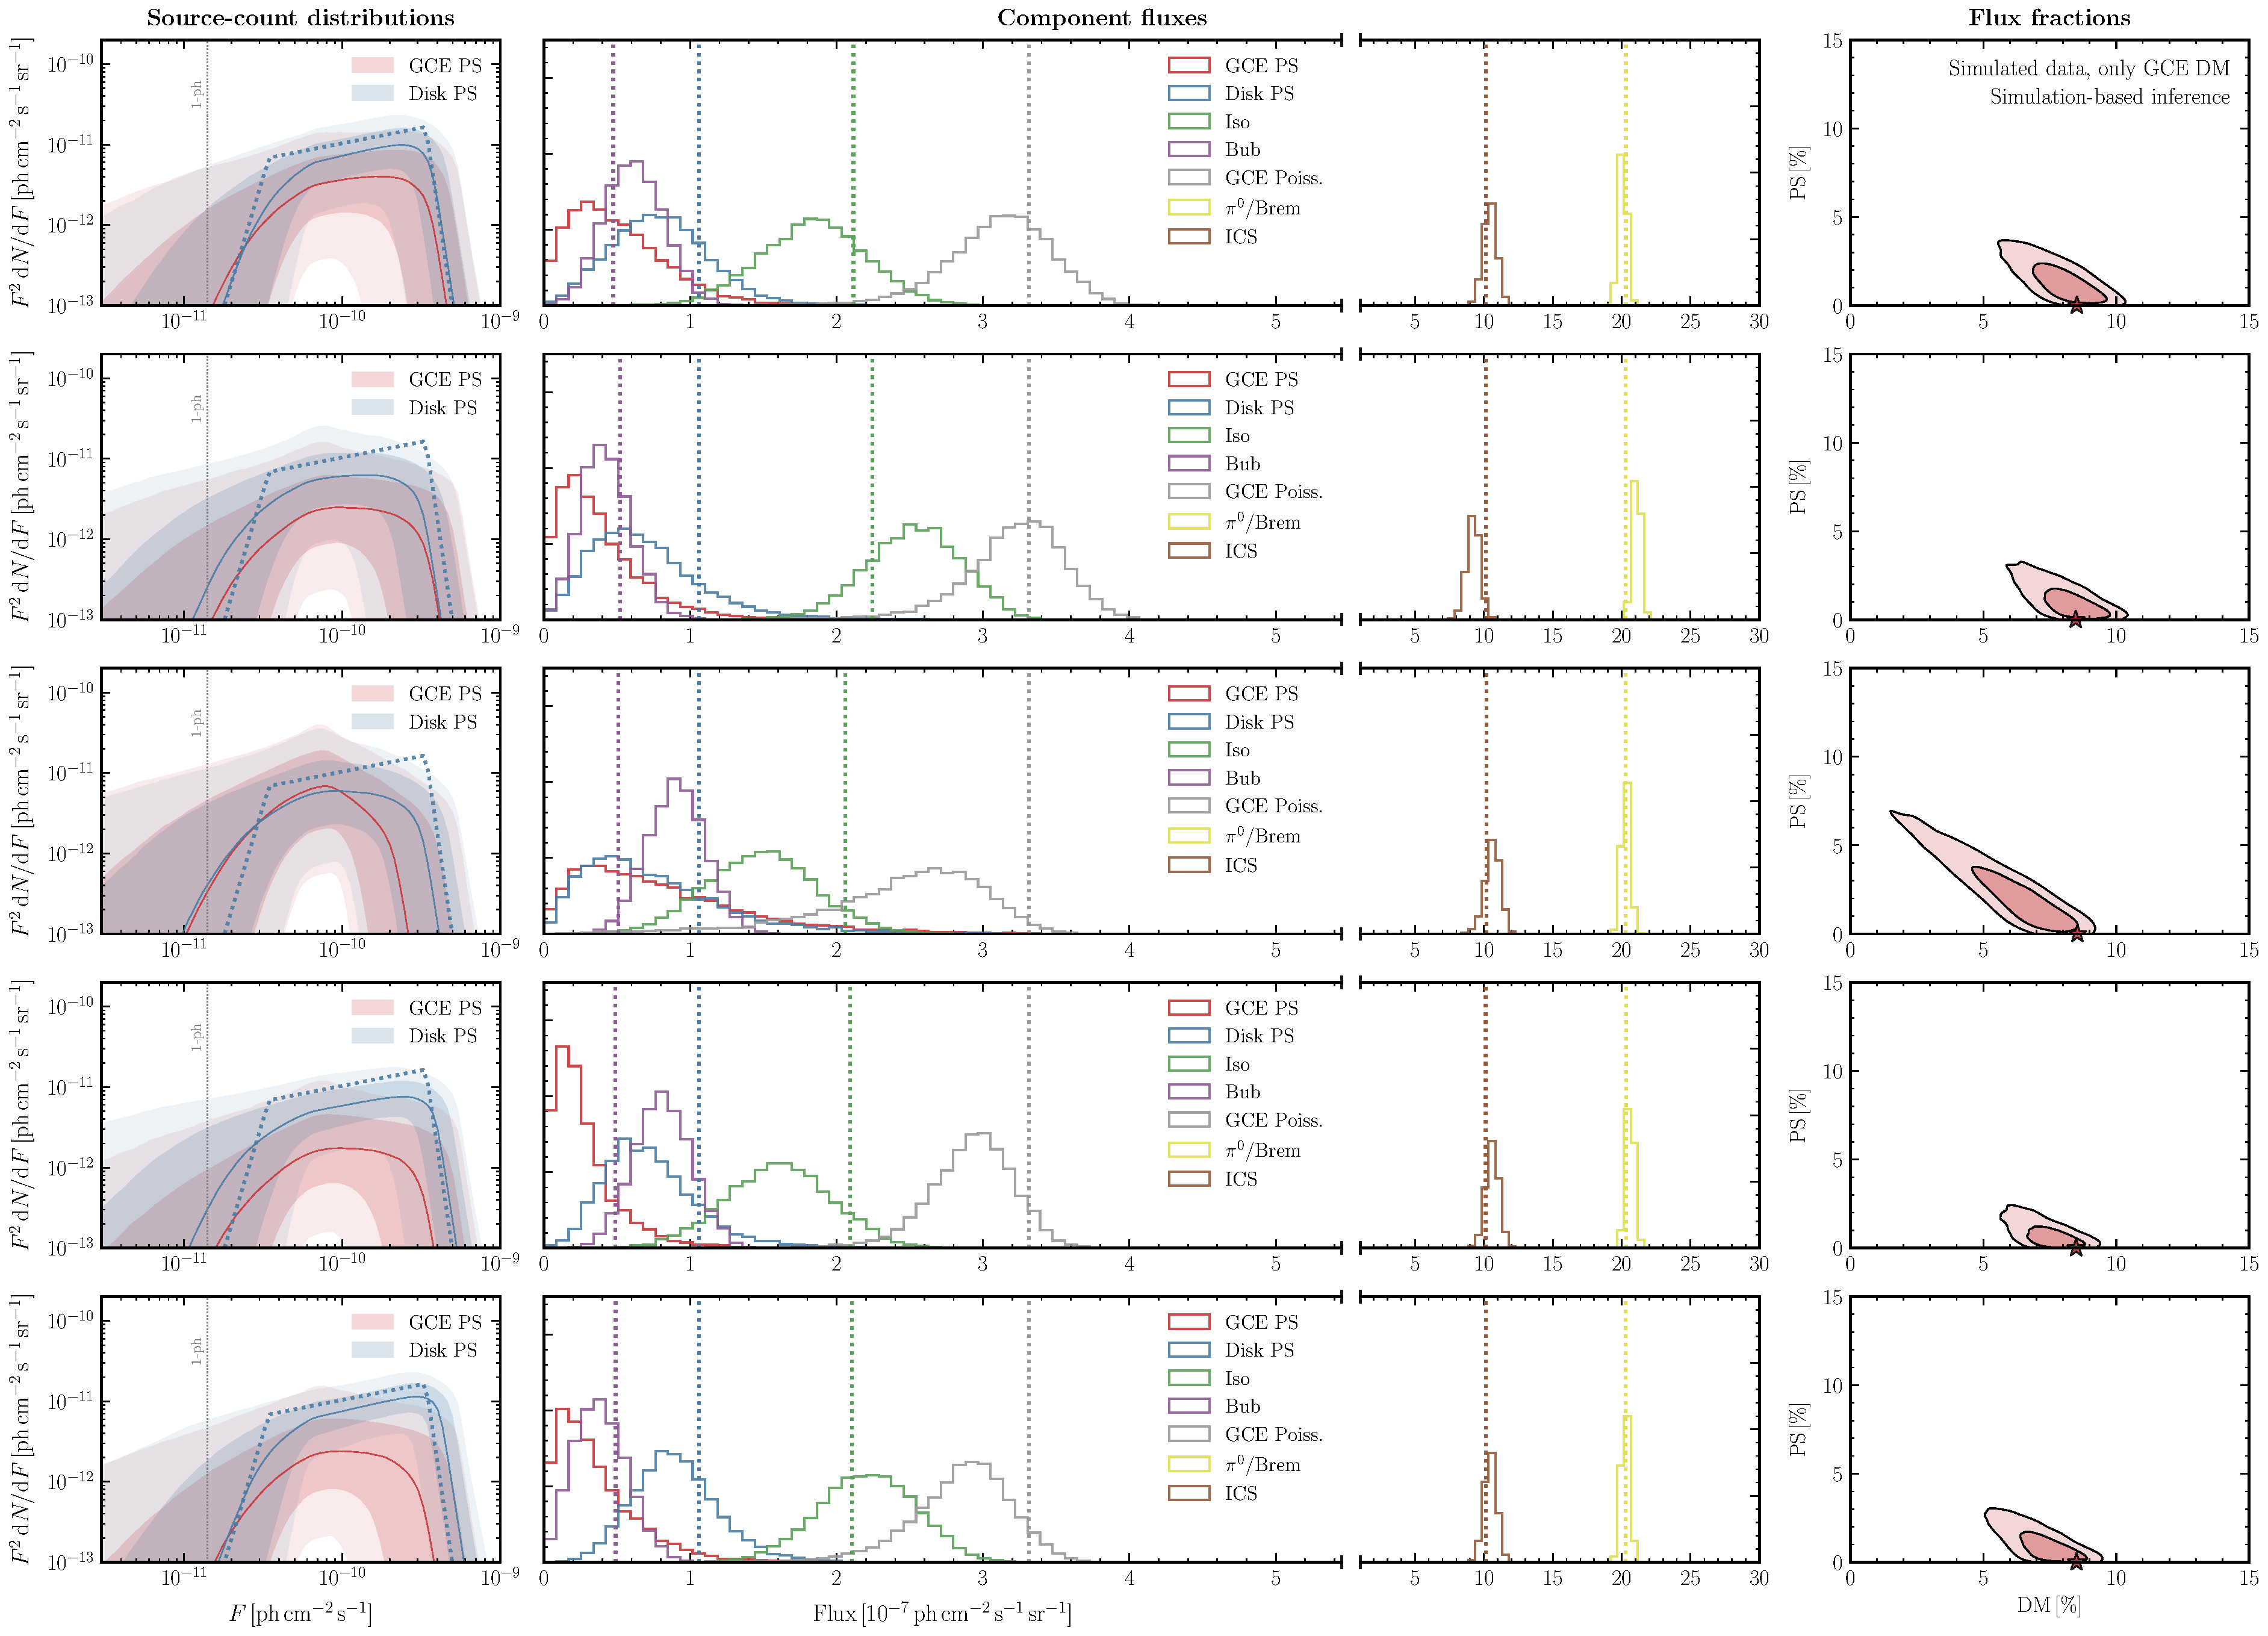
\includegraphics[width=0.95\textwidth]{plots/sim_sbi_dm.pdf}
    \caption{Results on simulated data where the GCE consists of purely DM-like emission, with different rows corresponding to different simulated realizations. The left column shows the inferred source-count distribution for GCE-correlated (red) and disk-correlated (blue) PS. The middle panel shows the posteriors for the Poissonian templates. The right panel shows the joins posterior on DM-like and PS-like emission. The dotted lines corresponding to the true simulated quantities in each panel. DM-like emission is inferred in each case, with the other posteriors corresponding well to their true simulated values.} 
    \label{fig:sim_sbi_dm}
\end{figure*}
%

\section{Tests on simulated data}
\label{sec:simulations}

We begin by validating our trained model on simulated data. We create simulated datasets using the best-fit astrophysical model obtained from a non-Poissonian fit in our fiducal ROI, and test the ability of our model to infer the presence of either DM-like or PS-like signals on top of this background.

Figure~\ref{fig:sim_sbi_dm} shows results on maps where the GCE consists of purely DM-like emission. The left column shows the middle-68/95\% containment of the point-wise posterior on the source-count distributions of GCE- and disk-correlated point source emission in red and blue, respectively. The middle column shows the posterior on emission of all components in our model. The right- column shows the fraction of DM- and PS-like emission in proportion to the total inferred flux in the ROI. The true underlying quantities from which the data was generated are represented by dotted lines. We see that, in all cases shown, we are successfully able to infer the presence of DM-like emission. Some PS-like emission is inferred in most cases as well, due to a combination of degeneracy with both disk-correlated and DM-like flux. The overall flux of all components corresponds well to their true underlying values.

Figure~\ref{fig:sim_sbi_ps} shows the corresponding results for simulated data containing PS-like emission. We see that PS-like emission is successfully inferred in each case. Furthermore, the model is able to characterize the source-count of PSs through the source count distribution. Some degeneracy with disk-like source is seen.

%
\begin{figure*}
    \centering
    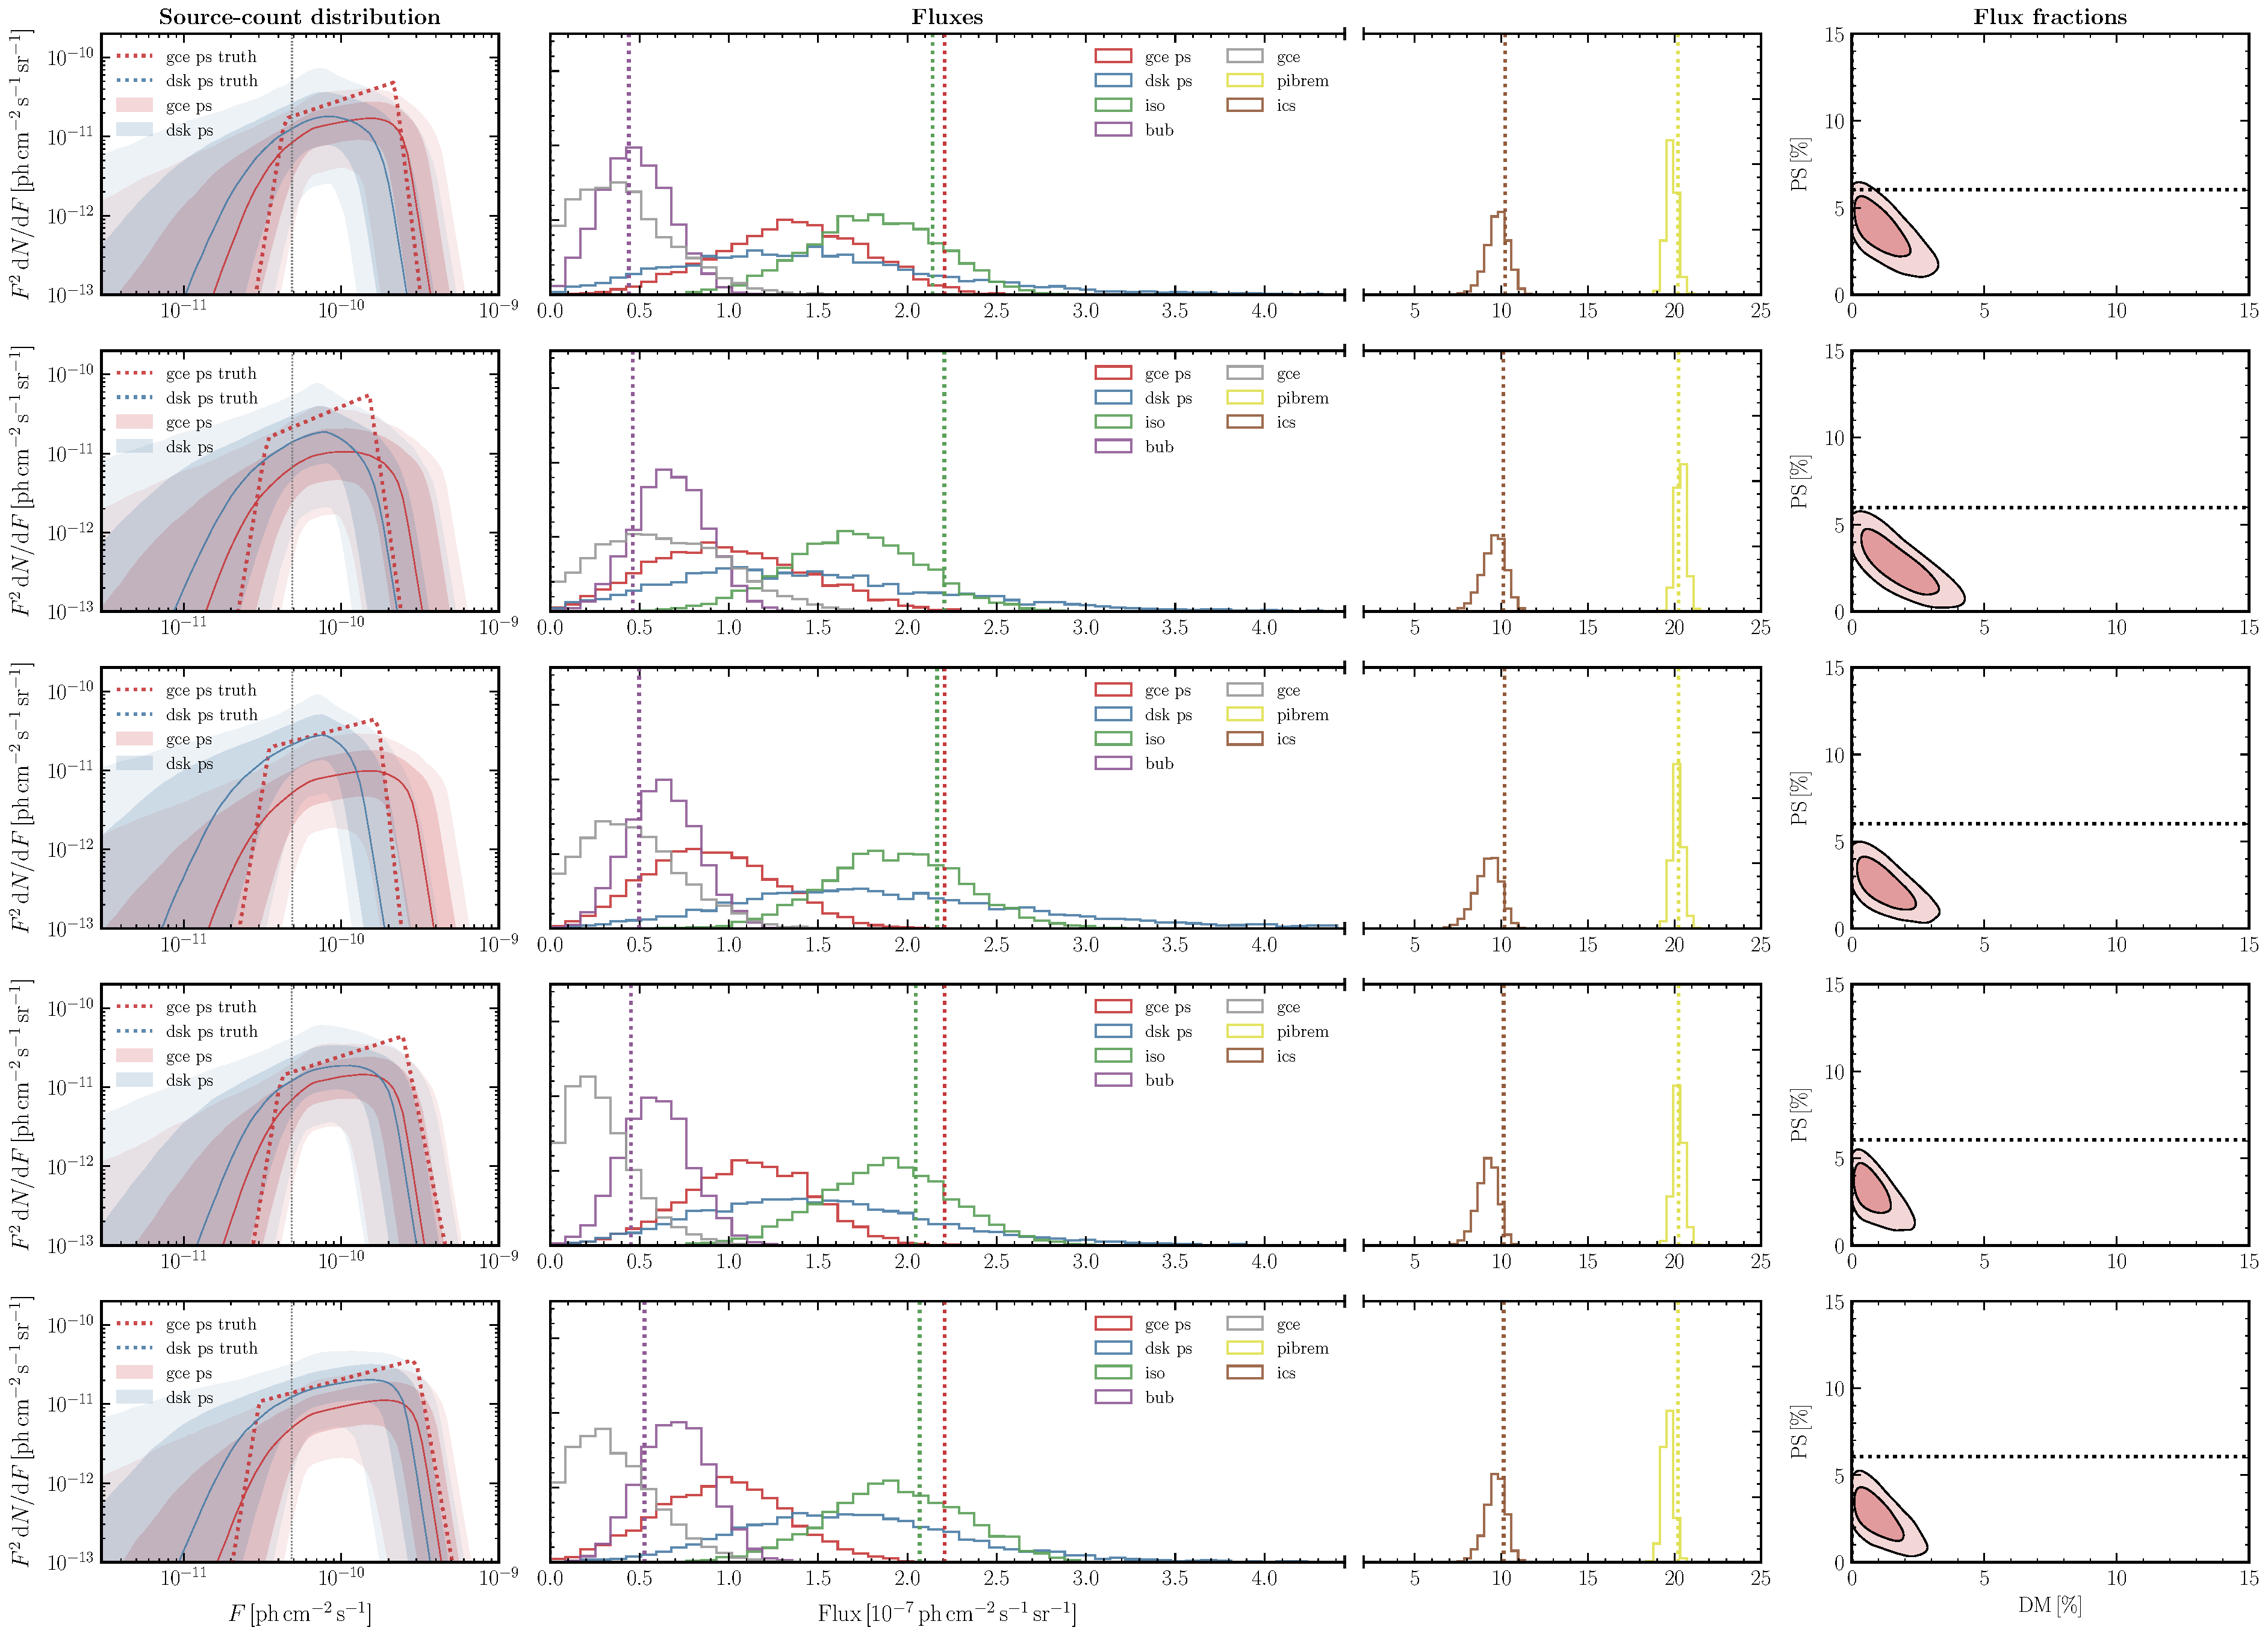
\includegraphics[width=0.95\textwidth]{plots/sim_sbi_ps.pdf}
    \caption{Same as Fig.~\ref{fig:sim_sbi_dm}, but for simulated data where the GCE consists of purely PS-like emission. PS-like emission is inferred in each case, with the other posteriors corresponding well to their true simulated values.}
    \label{fig:sim_sbi_ps}
\end{figure*}
%

\section{Results on \emph{Fermi} data}
\label{sec:data}

We finally apply our formalism to real \Fermi data. As a point of comparison, we also run the NPTF pipeline on the data using the same spatial templates and prior assumptions described in Sec.~\ref{sec:datasets}. The NPTF likelihood implemented in \texttt{NPTFit} from Ref.~\cite{Mishra-Sharma:2016gis} was used, and the posterior distribution was constructed through nested sampling using \texttt{dynesty} with 500 live points. The results of this analysis are shown in the bottom panel of Fig.~\ref{fig:fid_data}. Consistent with previous analyses using a similar configuration, a preference for PS-like emission is seen.

The top panel of Fig.~\ref{fig:fid_data} shows results using the neural simulation-based analysis pipeline. Although posteriors for the astrophysical background templates are seen to be broadly consistent with the NPTF anlaysis, No strong preference for PS-like emission is seen in this case. In fact, a near-exact degeneracy between DM-like and PS-like emission is seen.

%
\begin{figure*}
    \centering
    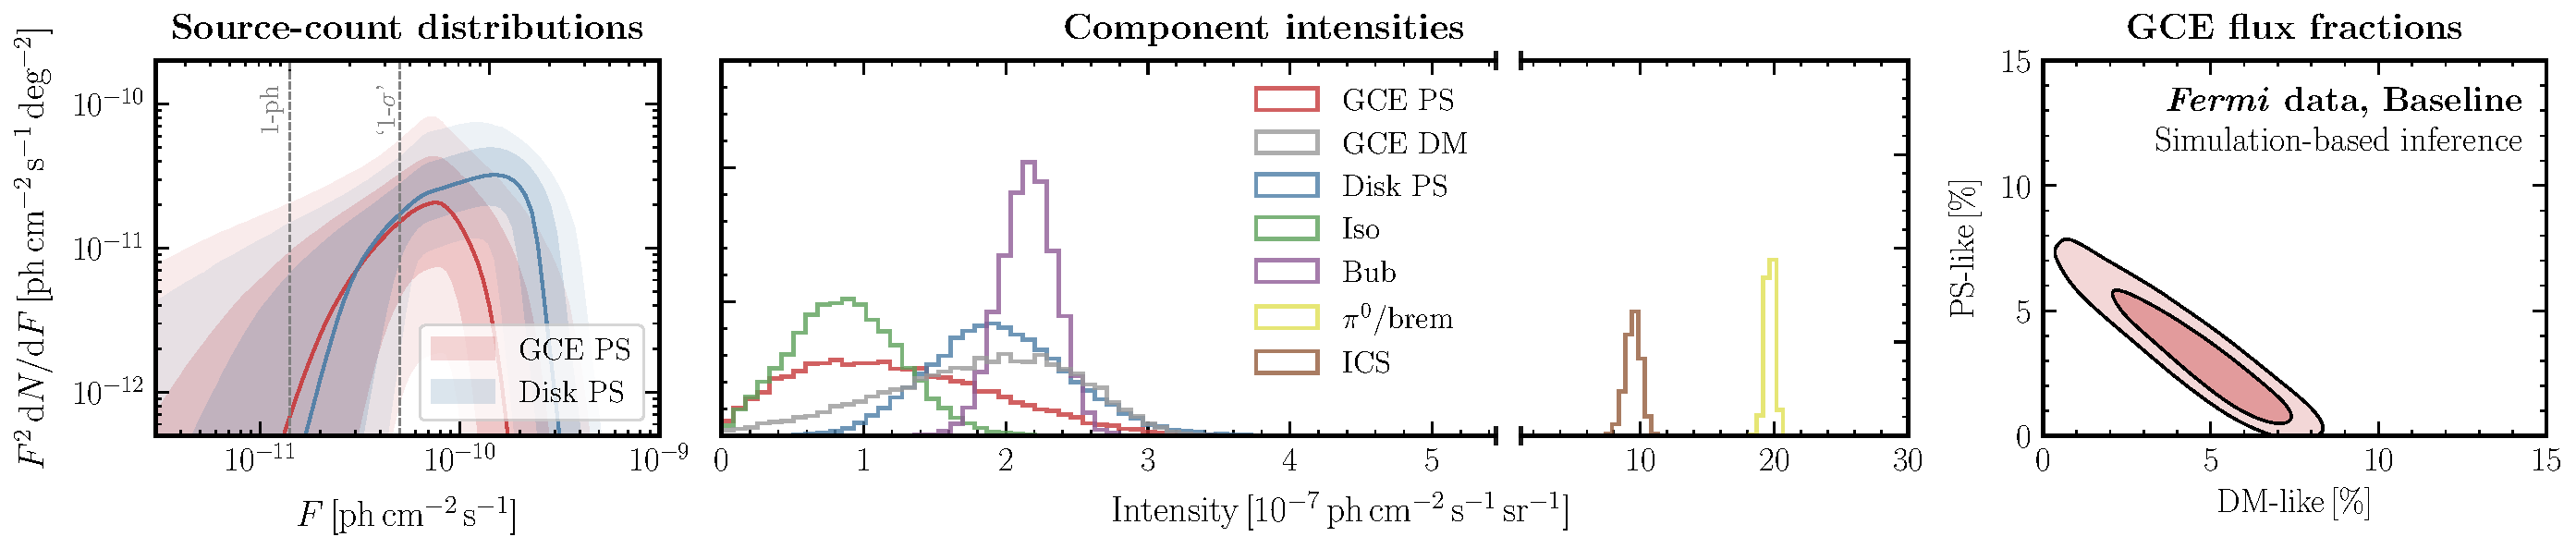
\includegraphics[width=0.95\textwidth]{plots/data_fid_sbi.pdf}
    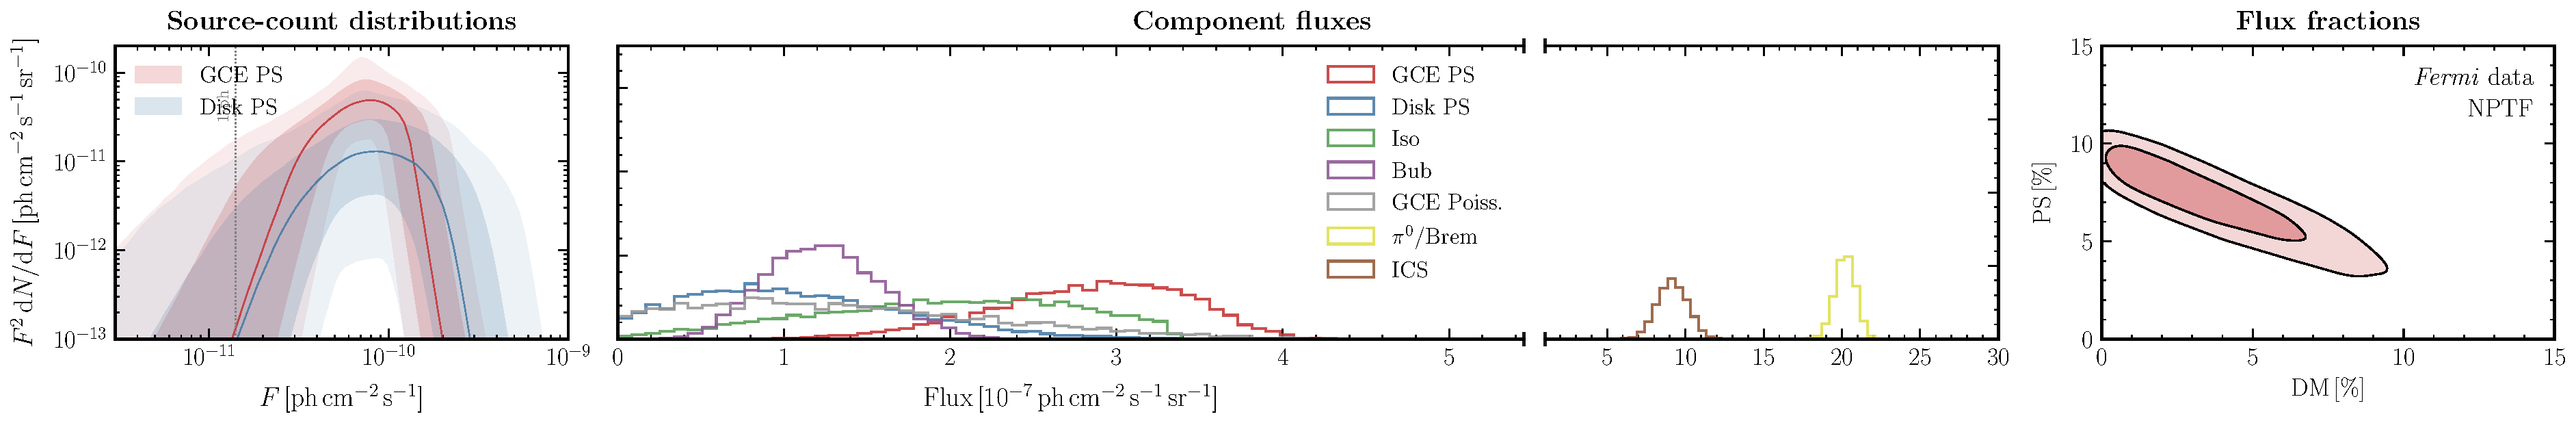
\includegraphics[width=0.95\textwidth]{plots/data_fid_nptf.pdf}
    \caption{Results of the fiducial analysis on data, with the top row corresponding to those obtained using the neural simulation-based inference pipeline, and the botton row using NPTF. While moderate preference for a PS-like origin of the GCE is seen in the case of the NPTF analysis, the SBI analysis finds a nearly perfect degeneracy between smooth and PS-like emission.}
    \label{fig:fid_data}
\end{figure*}
%

\subsection{Signal injection test}
\label{sec:sig-injection}

A crucial self-consistency test is the ability of the analysis to recover an artificial signal injected onto the real $\gamma$-ray data. Figure~\ref{fig:sig_inj_data} shows the joint posterior for flux fraction of PS-like and DM-like emission when an artificial DM signal is injected onto the real data. The leftmost panel shows the fiducial analysis on \Fermi data, with subsequent panels showing DM of varying normalizations injected onto the data. The dotted lines show the expected total emission on top of the median initial inferred flux. The additional DM is seen to be reconstructed correctly.

%
\begin{figure*}
    \centering
    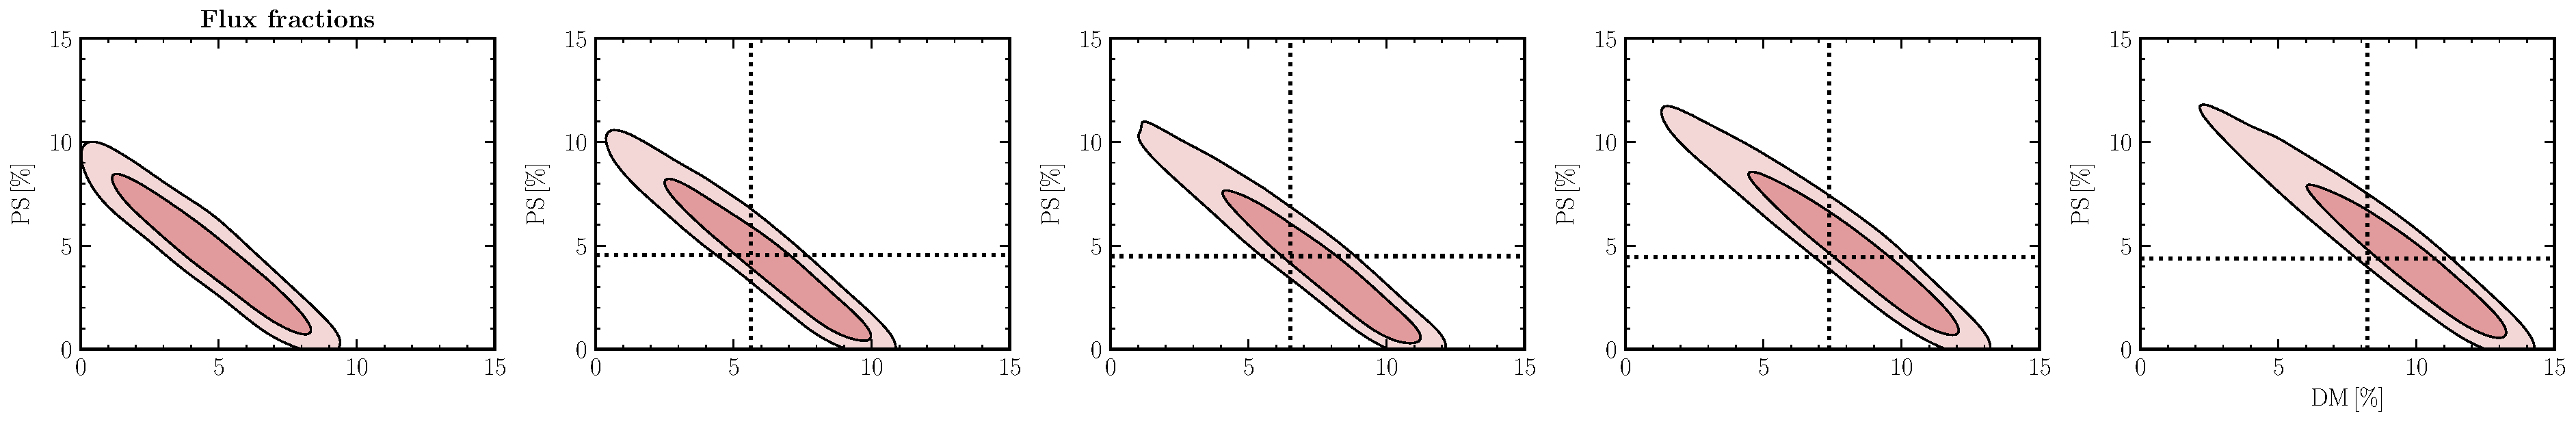
\includegraphics[width=0.95\textwidth]{plots/data_sig_inj.pdf}
    \caption{Joint posterior for flux fraction of PS-like and DM-like emission when an artificial DM signal is injected onto the real data. The leftmost panel shows the fiducial analysis on \Fermi data, with subsequent panels showing DM of varying normalizations injected onto the data. The dotted lines show the expected total emission on top of the median initial inferred flux. The additional DM is seen to be reconstructed correctly.}
    \label{fig:sig_inj_data}
\end{figure*}
%

\subsection{Systematic variations on analysis}
\label{sec:systematics}

%
\begin{figure}
    \centering
    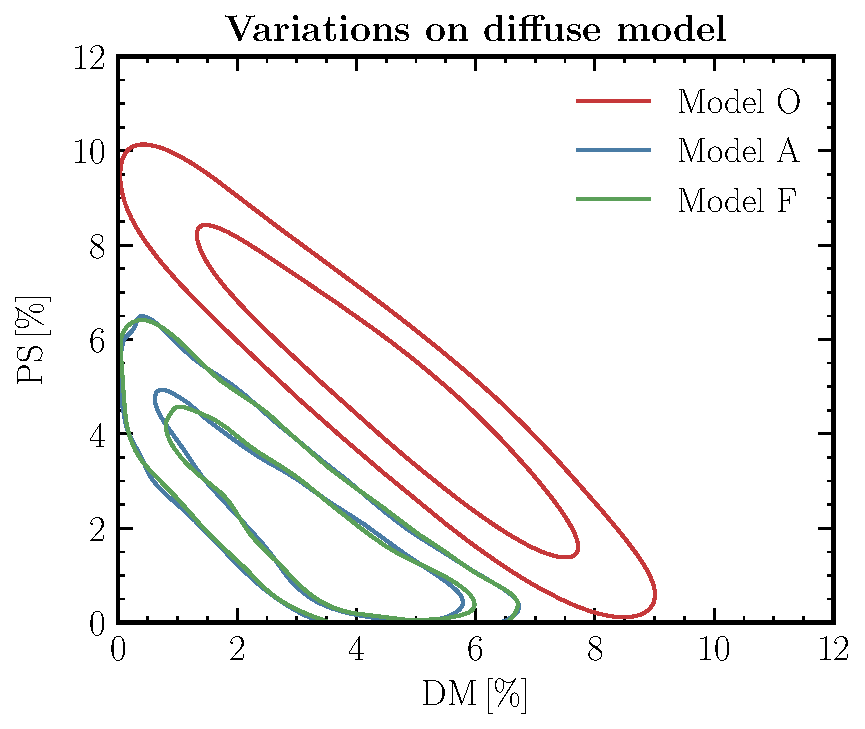
\includegraphics[width=0.22\textwidth]{plots/dif_var.pdf}
    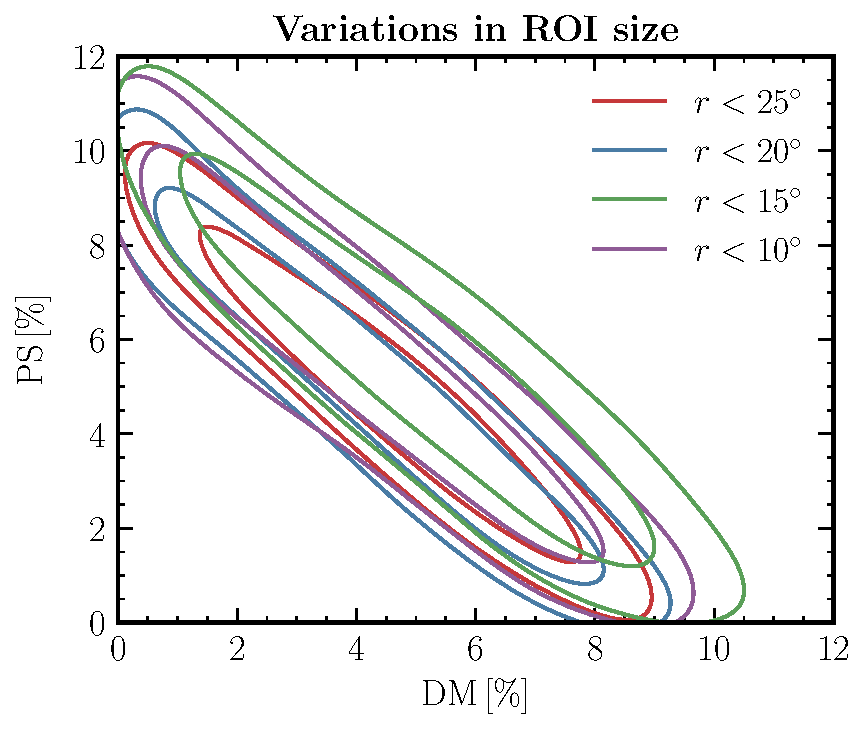
\includegraphics[width=0.22\textwidth]{plots/roi_var.pdf}
    \caption{Joint posterior for flux fraction of PS-like and DM-like emission on real \Fermi data for different diffuse models (left) and ROI sizes (right). In varying diffuse models, the fiducial Model O (red) is compared with results obtained using Models A (blue) and F (green). Although the overall GCE flux is seen to varying by up to a factor of $\sim2$ between diffuse models, no evidence for PS-like emission is seen. As seen in the right panel, results remain consistent for smaller ROI sizes.}
    \label{fig:variations}
\end{figure}
%

We explore several systematic variations of the fiducial analysis, shown in Fig.~\ref{fig:variations}.

\begin{itemize}
    \item \emph{Variation of the diffuse foreground model:} In addition to diffuse Model O considered in the fiducial analysis, we consider Models A and F from Ref.~\cite{} to model the diffuse foreground emission. Results for these variations are shown in the left panel of Fig.~\ref{fig:variations} for Models A (blue) and F (green) compared to the fiducial Model O (red). Although the overall GCE flux is seen to varying by up to a factor of $\sim2$ between diffuse models, no evidence for PS-like emission is seen using the additional diffuse models. A slight preference for smooth emission is seen for Models A and F, and the results between these two models and broadly similar. 
    \item \emph{Variations on the ROI size:} Although the GCE signal is concentrated predominantly in the inner $10^\circ$, the larger $25^\circ$ ROI used in this work may better constrain various emission components. However, there is also the potential for more susceptibility to mismodeling effects when using a larger ROI. The right panel of Fig.~\ref{fig:variations} shows analysis results using small ROI sizes---$10^\circ, 15^\circ$ and $20^\circ$. These are seen to be completely consistent with the fiducial analysis in the $25^\circ$ ROI.
\end{itemize}

% \begin{itemize}
%     \item Different diffuse models (Models A, B, F, p6v11, mismodeling, GP data-driven)
%     \item Different ROIs (15, 20, 25)
%     \item Varying inner slope of NFW profile
%     \item Different disk templates
% \end{itemize}

\section{Susceptibility to mismodeling}
\label{sec:mismodeling}

A key challenge associated with Galactic Center analyses is that associated with effects of mismodeled signal and background templates. In this section we assess the susceptibility of our simulation-based inference pipeline towards these systematics by constructing a data-driven model of large-scale mismodeling and assessing the ability of our method to recover either smooth or PS-like emission in the face of such mismodeling. 

Following Ref.~\cite{Mishra-Sharma:2020kjb}, we perform a Poissonian template analysis on the \Fermi dataset $d$, modulating the diffuse model template $T_{\mathrm{dif}}$ as described by the bremsstrahlung and neutral pion decay components of diffuse Model O by an (exponentiated) Gaussian process (GP):
\begin{equation}
    d \sim \operatorname{Pois}\left(\sum_{i \neq \mathrm{dif}} A_{i} T_{i}+\exp \left(f\right) A_{\mathrm{dif}} T_{\mathrm{dif}}\right).
\end{equation}
The other Poissonian templates $T_{i}$ are treated as before using an overall normalization factor $A_{i}$. $f \sim \mathcal{N}(m, K)$ is the GP component with mean $m$ set to zero, and the covariance $K$ described through the Mat\'ern kernel with smoothness parameter $\nu = 5/2$. We refer to Ref.~\cite{Mishra-Sharma:2020kjb} for further details of the analysis, as well a validation of the pipeline on simulated data.

%
\begin{figure}
    \centering
    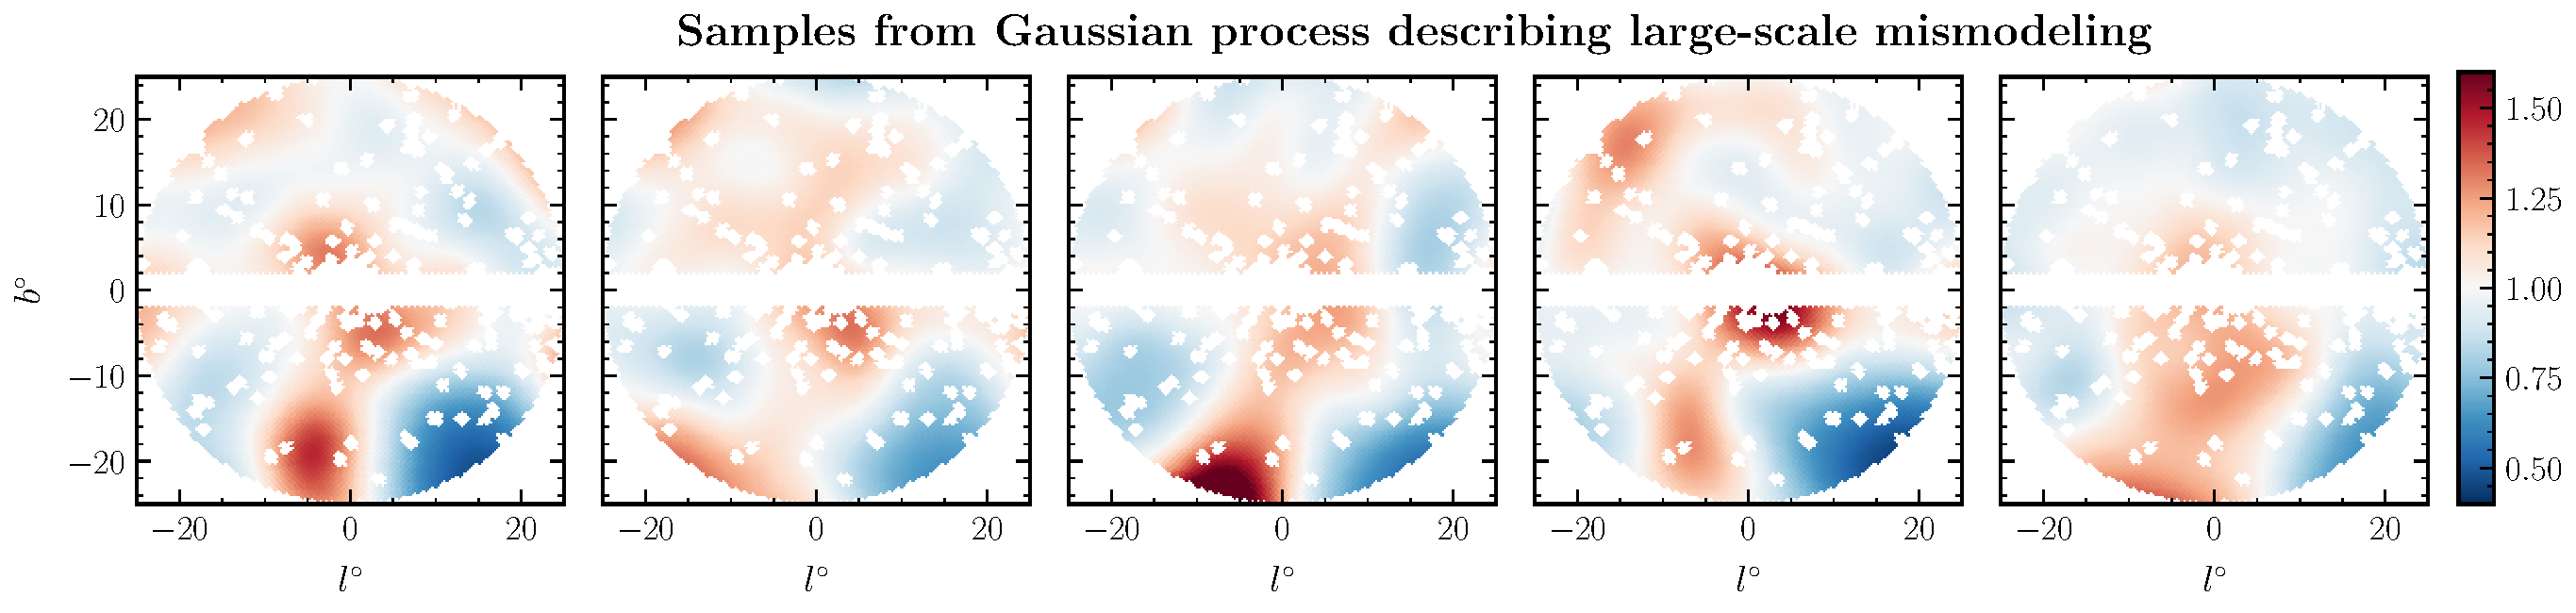
\includegraphics[width=0.45\textwidth]{plots/dd_mismo_map.pdf}
    \caption{The median Gaussian process description of multiplicative mismodeling associated with diffuse foreground Model O when applied to the real \Fermi data.}
    \label{fig:dd_mismo_map}
\end{figure}
%

The median Gaussian process describing the multiplicative mismodeling obtained relative to the real \Fermi data when using our fiducial diffuse Model O is shown in Fig.~\ref{fig:dd_mismo_map}. The most severe mismodeling is seen to be concentrated in the central and southern regions of the fiducial ROI. We modulate the bremsstrahlung and neutral pion decay-tracing components of Model O by this map, producing simulated data with the aim of mocking up large-scale mismodeling. These simulated samples are then analyzed with our standard pipeline, using the unmodulated diffuse model.

The results for this test are shown in Figs.~\ref{fig:sim_sbi_dm_mismo} and \ref{fig:sim_sbi_ps_mismo}, for simulated samples consisting of purely DM-like and PS-like emission, respectively. It can be seen that while large-scale mismodeling can distort the total flux attributed to either DM or PS-like emission, preference for the true underlying nature of the signal remains robust in either case. We note that the test with data-driven mismodeling tends to overestimate the DM flux, which may be attributed to the centrally-concentrated mismodeling as seen in Fig.~\ref{fig:dd_mismo_map}.

%
\begin{figure*}
    \centering
    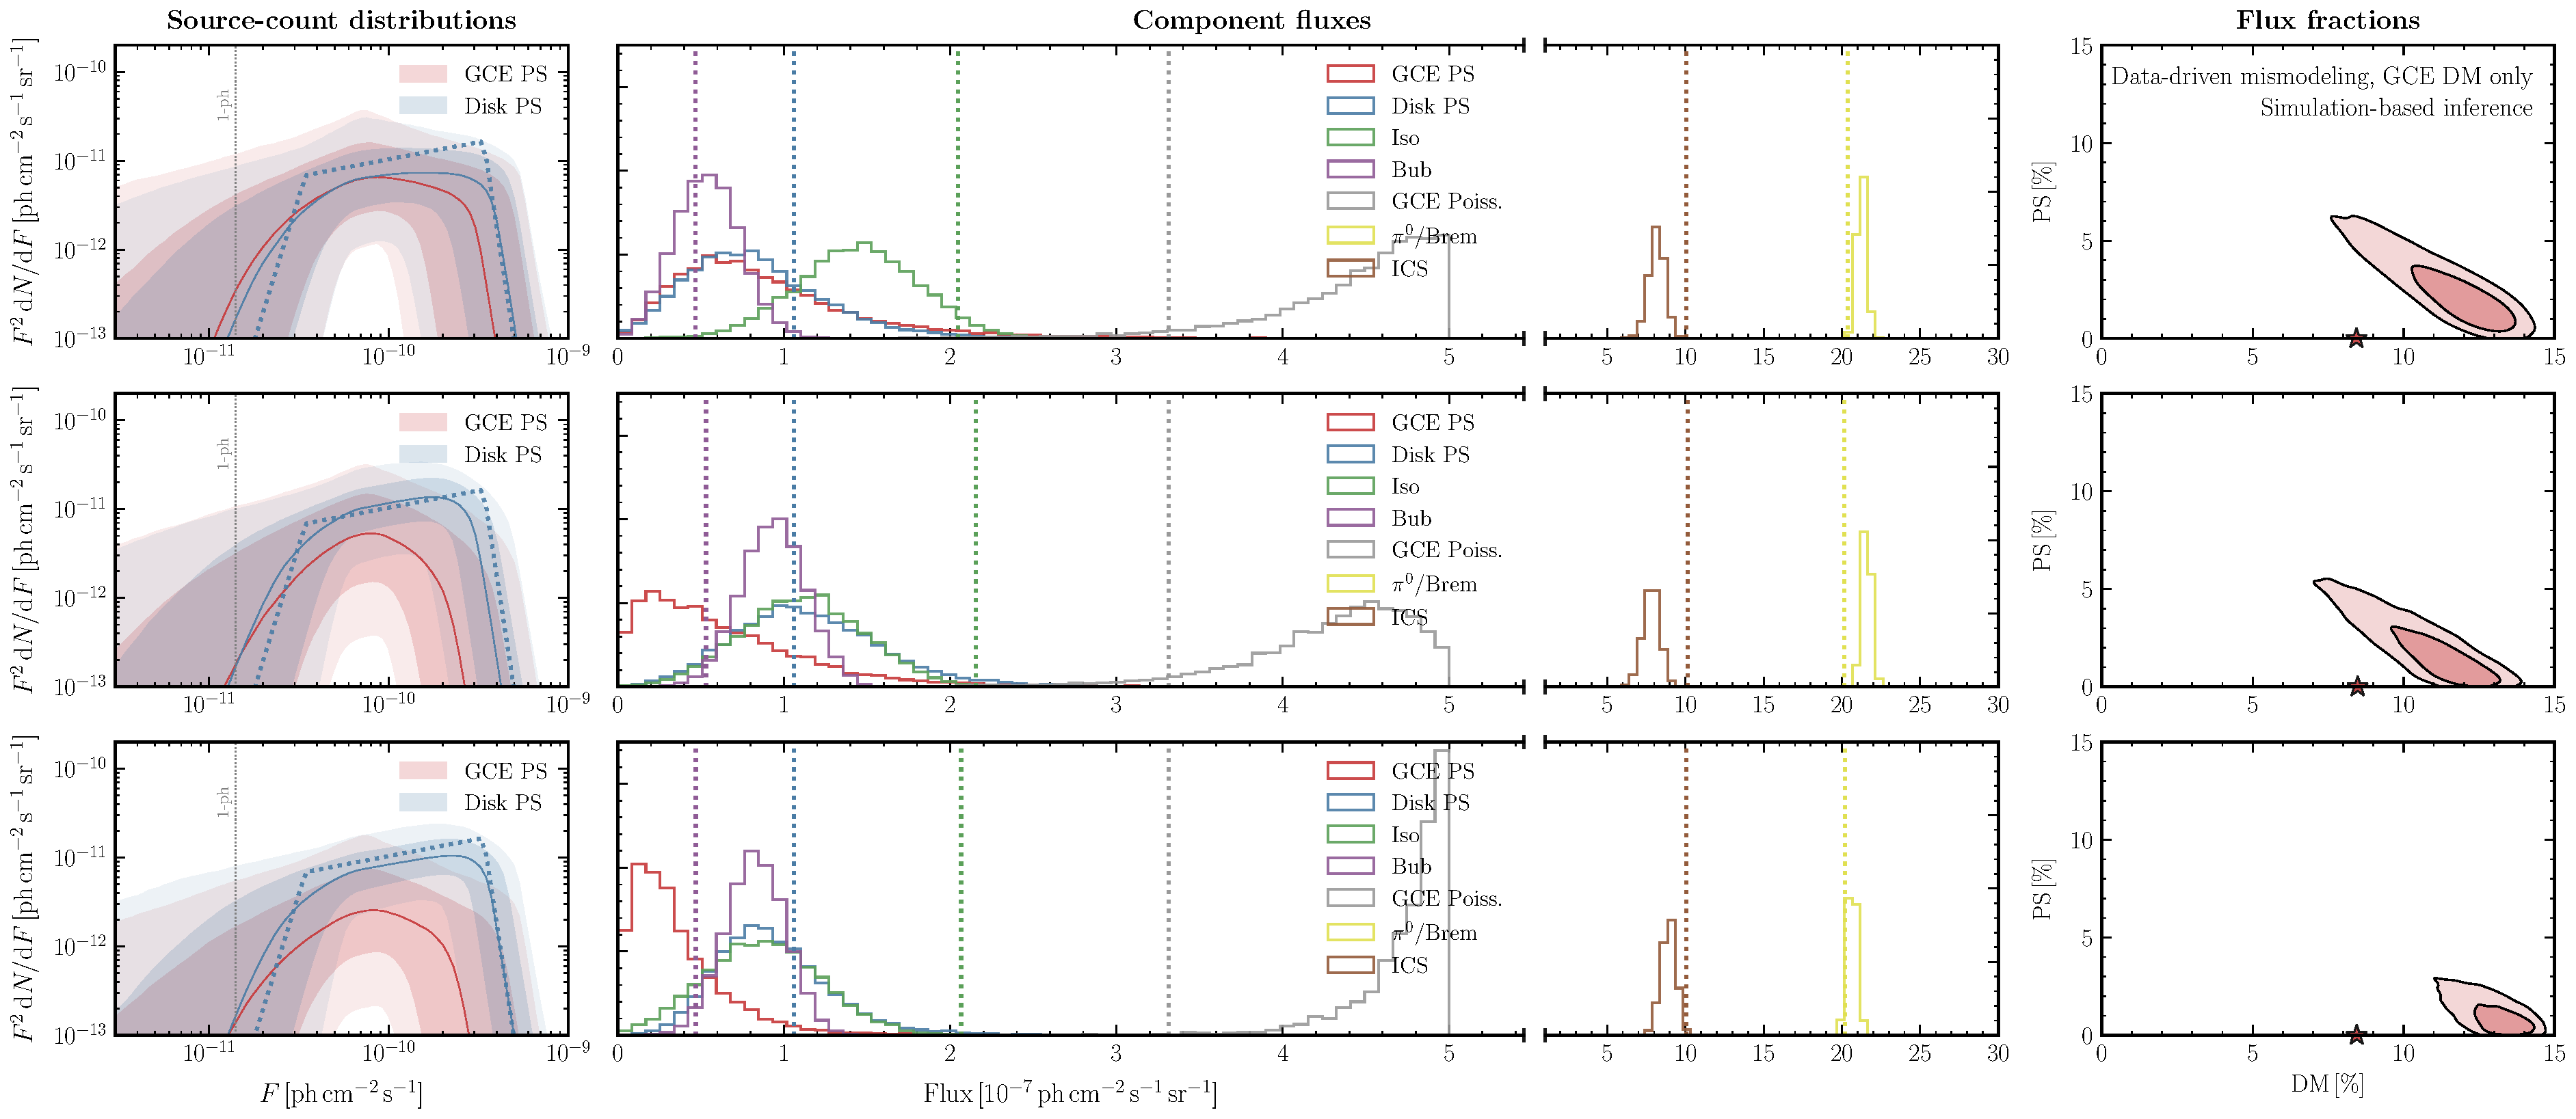
\includegraphics[width=0.95\textwidth]{plots/sim_sbi_dm_mismo.pdf}
    \caption{Same as Fig.~\ref{fig:sim_sbi_dm}, but for simulated data where the GCE consists of purely DM-like emission. DM-like emission is inferred in each case, with the other posteriors corresponding well to their true simulated values.}
    \label{fig:sim_sbi_dm_mismo}
\end{figure*}
%

%
\begin{figure*}
    \centering
    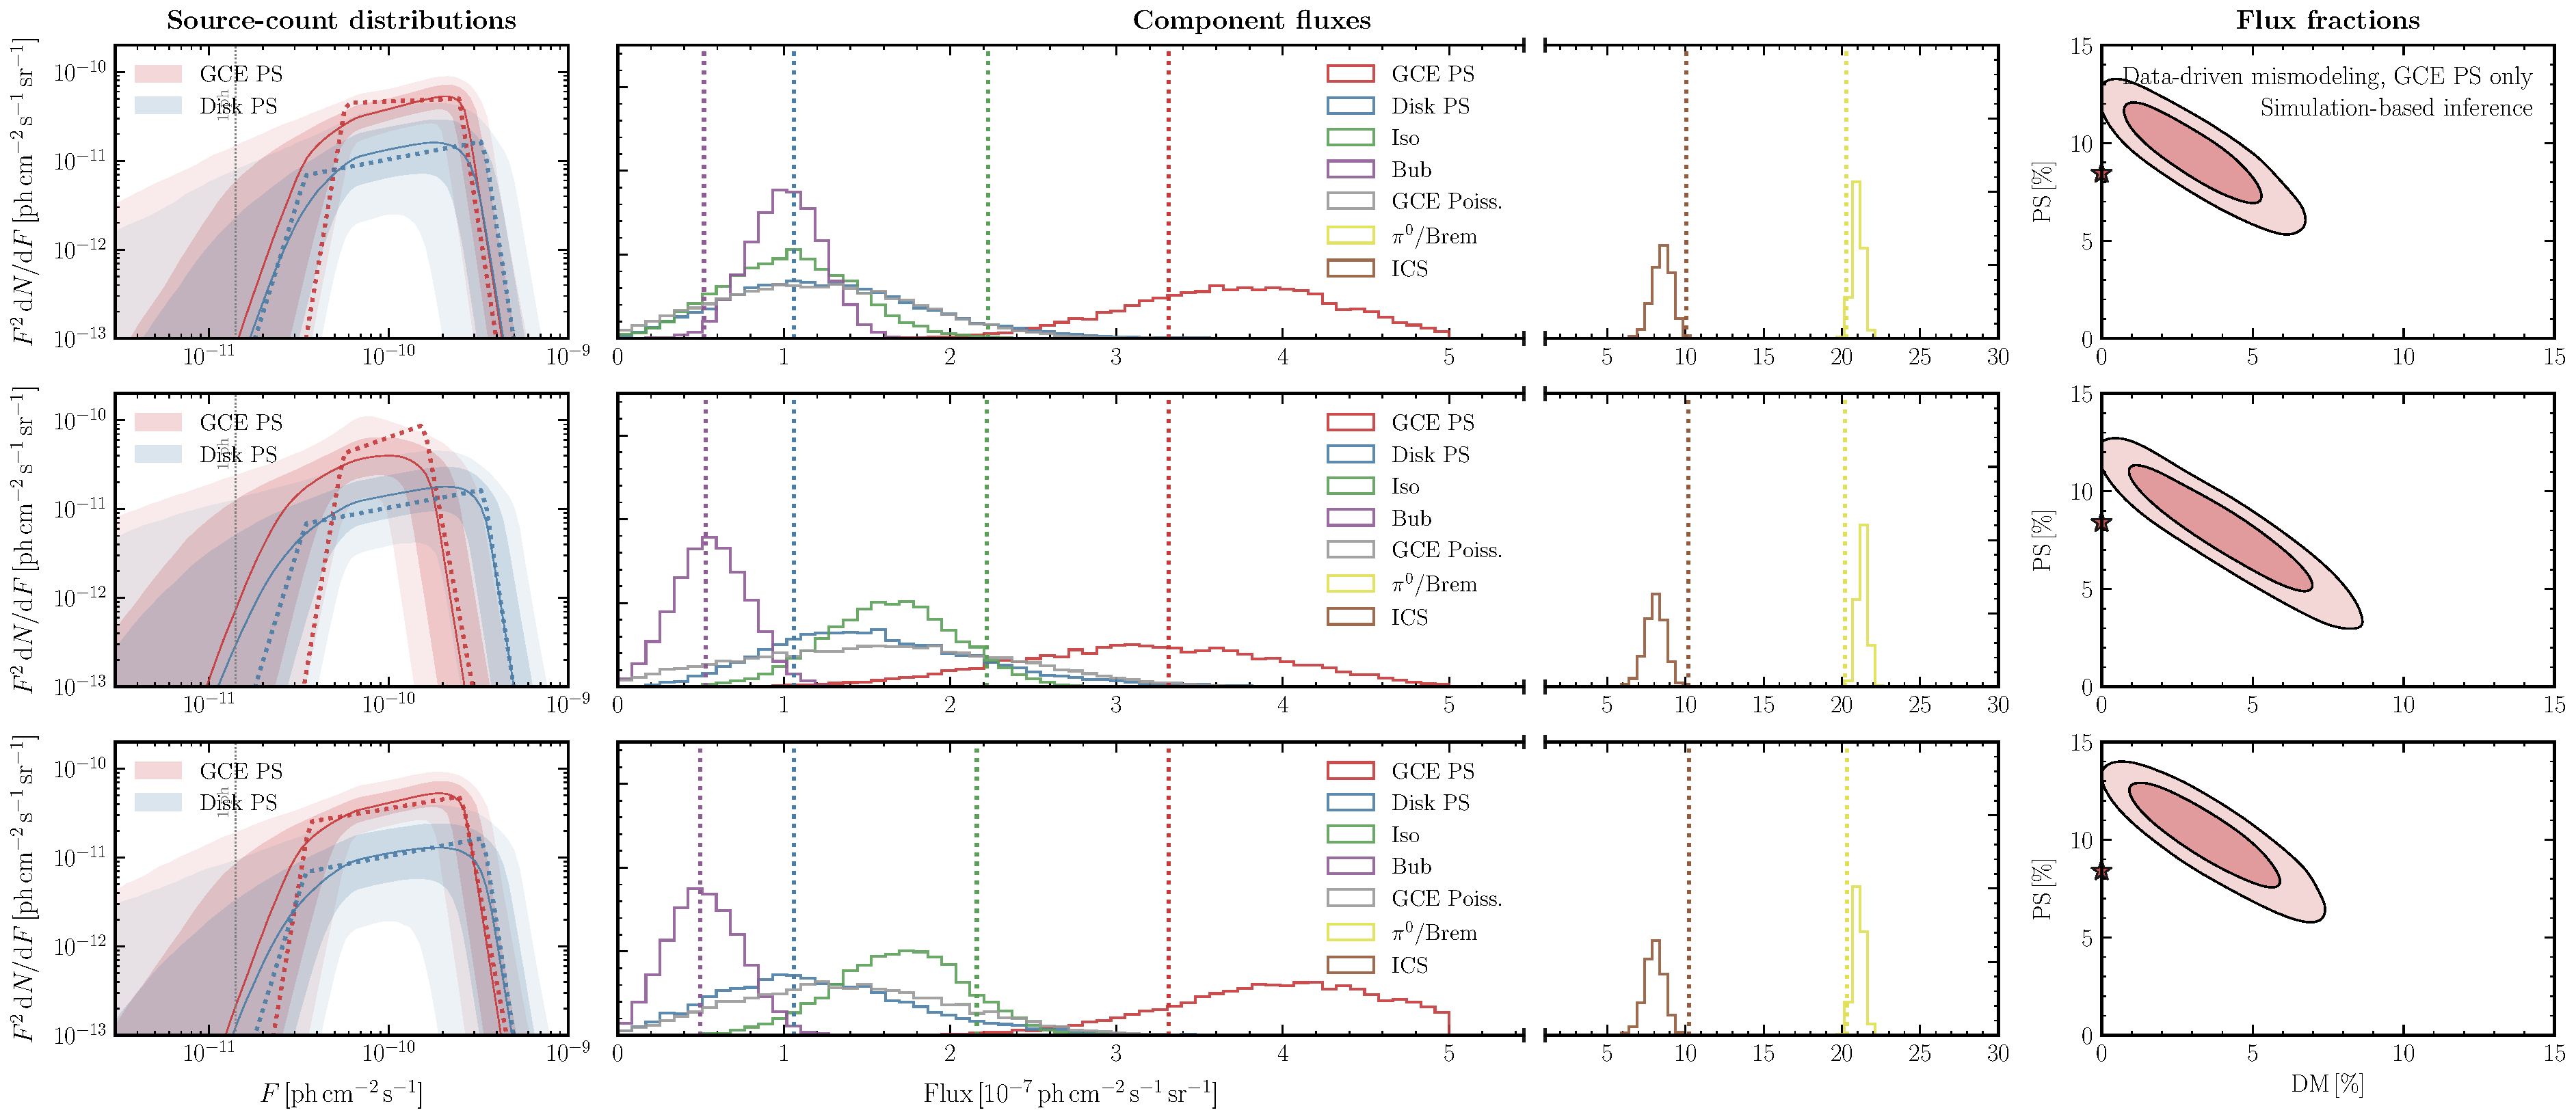
\includegraphics[width=0.95\textwidth]{plots/sim_sbi_ps_mismo.pdf}
    \caption{Same as Fig.~\ref{fig:sim_sbi_dm}, but for simulated data where the GCE consists of purely PS-like emission. PS-like emission is inferred in each case, with the other posteriors corresponding well to their true simulated values.}
    \label{fig:sim_sbi_ps_mismo}
\end{figure*}
%

\section{Discussion and Conclusions}
\label{sec:conclusion}

In this work, we have leveraged recent advances in neural simulation-based inference in order to weigh in on the nature of the \Fermi Galactic Center Excess. Consistent with the previous machine learning-based analysis of Ref~\cite{List:2020mzd}, our analysis based on conditional posterior density estimation with normalizing flows shows no substantive preference for a PS-like origin for a GCE signal across the systematic variations considered. We caution however of the potential of unknown systematics, such as small-scale diffuse mismodeling, mismodeling of the GCE signal itself, and unmodeled PS populations, to bias the conclusions of our study.

The code used to obtain the results in this paper is available at \url{https://github.com/smsharma/sbi-fermi}.

\vspace{.3cm}
%%%%%%%%%%%%%%%

\begin{acknowledgments}

We thank Johann Brehmer, Florian List, Nick Rodd, and Tracy Slatyer for helpful conversations.  
KC is partially supported by NSF awards ACI-1450310, OAC-1836650, and OAC-1841471, the NSF grant PHY-1505463, and the Moore-Sloan Data Science Environment at NYU. 
SM is supported by the NSF CAREER grant PHY-1554858, NSF grants PHY-1620727 and PHY-1915409, and the Simons Foundation. 
This work made use of the NYU IT High Performance Computing resources, services, and staff expertise. 
This research has made use of NASA's Astrophysics Data System. 
This research made use of the \texttt{astropy}~\cite{Price-Whelan:2018hus,Robitaille:2013mpa}, \texttt{dynesty}~\cite{Speagle_2020}, \texttt{IPython}~\cite{PER-GRA:2007}, Jupyter~\cite{Kluyver2016JupyterN}, \texttt{matplotlib}~\cite{Hunter:2007}, \texttt{MLflow}~\cite{chen2020developments}, \texttt{NPTFit}~\cite{Mishra-Sharma:2016gis}, \texttt{NumPy}~\cite{harris2020array}, \texttt{pandas}~\cite{pandas:2010}, \texttt{Pyro}, \texttt{PyTorch}~\cite{NEURIPS2019_9015}, \texttt{PyTorch Geometric}~\cite{Fey/Lenssen/2019}, \texttt{PyTorch Lightning}~\cite{william_falcon_2020_3828935}, \texttt{seaborn}~\cite{seaborn}, \texttt{sbi}~\cite{tejero-cantero2020sbi}, \texttt{scikit-learn}~\cite{scikit-learn}, \texttt{SciPy}~\cite{2020SciPy-NMeth}, and \texttt{tqdm}~\cite{da2019tqdm}  software packages. We acknowledge the use of the code repository associated with Ref.~\cite{List:2020mzd}, in particular the associated data products and templates.\footnote{\url{https://github.com/FloList/GCE_NN}}
\end{acknowledgments}

% \appendix

% \section{Variations on analysis}
% \label{app:variations}

\bibliographystyle{apsrev4-1}
\bibliography{fermi-gce-sbi}

\end{document}
